\section{Lecture 3: Camera Model, Triangulation, Point/Line/Plane}
\label{sec:lecture03}

\paragraph{Topics.} (1) camera measurements; (2) essential matrix / triangulation; (3) point / line / plane representations.

% Tighten matrix column spacing for the dense Jacobian/triangulation blocks in this lecture.
\setlength{\arraycolsep}{3.5pt}

% =====================================================================
% Reusable camera-projection scene (Figs. 1, 4, 5 share this geometry).
\newcommand{\camprojscene}{%
  % Camera frame {C}
  \draw[->,thick] (0,0) -- (0.9,0) node[right] {$x$};
  \draw[->,thick] (0,0) -- (0,-0.9) node[below] {$y$};
  \node[above left=-2pt] at (0,0) {$\{C\}$};
  \fill (0,0) circle (1.5pt);
  % Single optical ray {C} --(z_c)-- P_f: the pixel z_c is where the sight ray
  % pierces the image plane, so {C}, z_c, and P_f are collinear.
  \coordinate (lc3zc) at (1.515,0.90);   % = 0.30 * (5.05,3.00), on the ray
  \draw[thin,gray!70] (0,0) -- (lc3zc);
  \draw[dashed] (lc3zc) -- (5.05,3.00);
  % Image plane (blue, tilted parallelogram) centred on z_c, pierced by the ray
  \draw[blue,thick] (0.766,1.505) -- (1.426,1.705) -- (2.264,0.295) -- (1.604,0.095) -- cycle;
  \fill[blue] (lc3zc) circle (1.3pt);
  \node[blue,right=1pt] at (1.66,0.99) {$\vect{z}_c$};
  \node[left] at (0.55,1.78) {\footnotesize Image plane};
  % Feature point P_f
  \fill (5.05,3.00) circle (1.6pt);
  \node[above right] at (5.05,3.00) {$\vect{P}_f$};
  % C-frame sight line label: ^C p_f
  \node[above left] at (3.55,2.45) {${}^{C}\vect{p}_f$};
  % Global frame {G}
  \draw[->,thick] (6.20,0) -- (6.20,1.10) node[above] {$z$};
  \draw[->,thick] (6.20,0) -- (7.12,0.16) node[right] {$y$};
  \node at (5.88,-0.14) {$\boldsymbol{\times}$};
  \node[below] at (5.88,-0.22) {$x$};
  \node[above right=0pt] at (6.30,0.10) {$\{G\}$};
  \fill (6.20,0) circle (1.5pt);
  % Global ray to the feature: ^G p_f
  \draw[dotted,thick] (6.20,0) -- (5.05,3.00);
  \node[right] at (5.55,1.70) {${}^{G}\vect{p}_f$};
  % Red baseline between the two frames: extrinsic {^C_G R, ^C p_c}
  \draw[red,thick] (0,0) to[bend right=12] (6.20,0);
}

% =====================================================================
\subsection{The camera measurement model}

A camera produces pixel measurements that depend on the camera pose and the observed scene:
\begin{align}
\vect{z}_c = \vect{h}_c(\vect{x}) + \vect{n}_c,
\end{align}
where $\vect{z}_c$ are the pixel measurements, $\vect{x}$ is the state vector (camera pose and point feature), $\vect{h}_c(\cdot)$ is the camera model, and $\vect{n}_c$ is the pixel noise. The geometry is shown in Fig.~\ref{fig:lec03-cammodel}.

\begin{figure}[H]
\centering
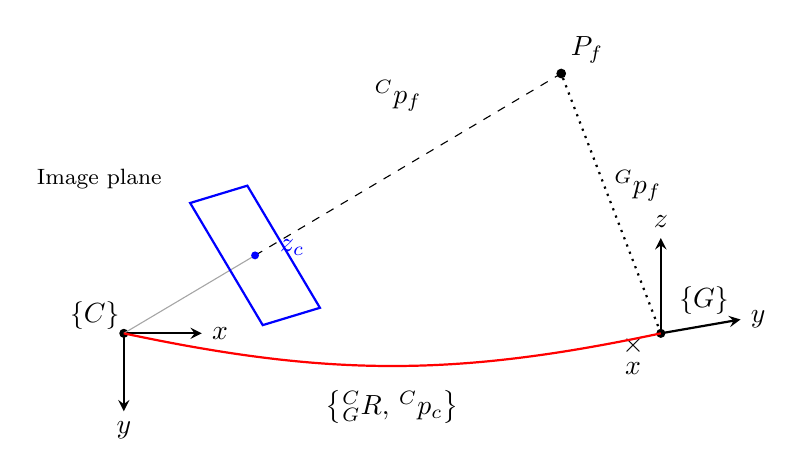
\begin{tikzpicture}[>=stealth,scale=1.1]
  \camprojscene
  \node[below] at (3.10,-0.55) {$\big\{{}^{C}_{G}\vect{R},\,{}^{C}\vect{p}_c\big\}$};
\end{tikzpicture}
\caption{Camera measurement geometry: the feature $\vect{P}_f$ projects through the image plane to the pixel $\vect{z}_c$ in the camera frame $\{C\}$; the global frame $\{G\}$ and the extrinsic $\{{}^{C}_{G}\vect{R},{}^{C}\vect{p}_c\}$ relate the two views of the same point (${}^{C}\vect{p}_f$ vs.\ ${}^{G}\vect{p}_f$).}
\label{fig:lec03-cammodel}
\end{figure}

\paragraph{Simplest pinhole model.} With the feature in the camera frame ${}^{C}\vect{p}_f = [x,\,y,\,z]\trans$, the normalized projection is
\begin{align}
\vect{z}_n = \begin{bmatrix} u_n \\ v_n \end{bmatrix} = \begin{bmatrix} x/z \\ y/z \end{bmatrix},
\qquad
\vect{z}_n = \vect{h}_p({}^{C}\vect{p}_f) + \vect{n}_c, \quad {}^{C}\vect{p}_f = {}^{C}_{G}\vect{R}\trans\big({}^{G}\vect{p}_f - {}^{G}\vect{p}_c\big).
\end{align}
Linearizing the measurement, $\tilde{\vect{z}}_n = \vect{H}_c\,\tilde{\vect{x}} + \vect{n}_c$, with the residual
\begin{align}
\tilde{\vect{z}}_n = \vect{z}_n - \vect{h}_p({}^{C}\hat{\vect{p}}_f) = \begin{bmatrix} u_n \\ v_n \end{bmatrix} - \begin{bmatrix} \hat{x}/\hat{z} \\ \hat{y}/\hat{z} \end{bmatrix}.
\end{align}
The state and its error state are
\begin{align}
\vect{x} : \big\{{}^{C}_{G}\vect{R},\,{}^{G}\vect{p}_c,\,{}^{G}\vect{p}_f\big\}, \quad
{}^{C}_{G}\vect{R} = {}^{C}_{G}\hat{\vect{R}}\,\Exp(\delta\vect{\theta}), \;\;
{}^{G}\vect{p}_c = {}^{G}\hat{\vect{p}}_c + {}^{G}\tilde{\vect{p}}_c, \;\;
{}^{G}\vect{p}_f = {}^{G}\hat{\vect{p}}_f + {}^{G}\tilde{\vect{p}}_f,
\end{align}
with error state $\tilde{\vect{x}} = [\,\delta\vect{\theta}\trans,\; {}^{G}\tilde{\vect{p}}_c\trans,\; {}^{G}\tilde{\vect{p}}_f\trans\,]\trans$.

% =====================================================================
\subsection{The measurement Jacobian}

By the chain rule, factoring every block through ${}^{C}\tilde{\vect{p}}_f$,
\begin{align}
\tilde{\vect{z}}_n &= \vect{H}_c\,\tilde{\vect{x}} + \vect{n}_c \\
&= \begin{bmatrix} \dfrac{\partial\tilde{\vect{z}}_n}{\partial\delta\vect{\theta}} & \dfrac{\partial\tilde{\vect{z}}_n}{\partial{}^{G}\tilde{\vect{p}}_c} & \dfrac{\partial\tilde{\vect{z}}_n}{\partial{}^{G}\tilde{\vect{p}}_f} \end{bmatrix}\tilde{\vect{x}} + \vect{n}_c \\
&= \frac{\partial\tilde{\vect{z}}_n}{\partial{}^{C}\tilde{\vect{p}}_f}\begin{bmatrix} \dfrac{\partial{}^{C}\tilde{\vect{p}}_f}{\partial\delta\vect{\theta}} & \dfrac{\partial{}^{C}\tilde{\vect{p}}_f}{\partial{}^{G}\tilde{\vect{p}}_c} & \dfrac{\partial{}^{C}\tilde{\vect{p}}_f}{\partial{}^{G}\tilde{\vect{p}}_f} \end{bmatrix}\tilde{\vect{x}} + \vect{n}_c.
\end{align}
The projection Jacobian, writing ${}^{C}\vect{p}_f = [c_x,\,c_y,\,c_z]\trans$, is
\begin{align}
\vect{z}_n = \begin{bmatrix} c_x/c_z \\ c_y/c_z \end{bmatrix}, \qquad
\frac{\partial\vect{z}_n}{\partial{}^{C}\vect{p}_f} = \begin{bmatrix} \dfrac{1}{c_z} & 0 & -\dfrac{c_x}{c_z^{2}} \\[2ex] 0 & \dfrac{1}{c_z} & -\dfrac{c_y}{c_z^{2}} \end{bmatrix}
= \frac{1}{c_z^{2}}\begin{bmatrix} c_z & 0 & -c_x \\ 0 & c_z & -c_y \end{bmatrix}.
\end{align}

\paragraph{Perturbing ${}^{C}\vect{p}_f$.} From ${}^{C}\vect{p}_f = {}^{C}_{G}\vect{R}\trans({}^{G}\vect{p}_f - {}^{G}\vect{p}_c)$ with ${}^{C}_{G}\vect{R} = {}^{C}_{G}\hat{\vect{R}}\,\Exp(\delta\vect{\theta})$ and $\Exp(\delta\vect{\theta})\trans \approx \vect{I} - \skewsym{\delta\vect{\theta}}$,
\begin{align}
{}^{C}\hat{\vect{p}}_f + {}^{C}\tilde{\vect{p}}_f
&= \big({}^{C}_{G}\hat{\vect{R}}\,\Exp(\delta\vect{\theta})\big)\trans\big({}^{G}\hat{\vect{p}}_f + {}^{G}\tilde{\vect{p}}_f - {}^{G}\hat{\vect{p}}_c - {}^{G}\tilde{\vect{p}}_c\big) \\
&= \big(\vect{I} - \skewsym{\delta\vect{\theta}}\big)\,{}^{C}_{G}\hat{\vect{R}}\trans\big({}^{G}\hat{\vect{p}}_f + {}^{G}\tilde{\vect{p}}_f - {}^{G}\hat{\vect{p}}_c - {}^{G}\tilde{\vect{p}}_c\big) \\
&\approx {}^{C}_{G}\hat{\vect{R}}\trans\big({}^{G}\hat{\vect{p}}_f - {}^{G}\hat{\vect{p}}_c\big) - \skewsym{\delta\vect{\theta}}\,{}^{C}_{G}\hat{\vect{R}}\trans\big({}^{G}\hat{\vect{p}}_f - {}^{G}\hat{\vect{p}}_c\big) \notag\\
&\quad + {}^{C}_{G}\hat{\vect{R}}\trans\big({}^{G}\tilde{\vect{p}}_f - {}^{G}\tilde{\vect{p}}_c\big).
\end{align}
Using $-\skewsym{\delta\vect{\theta}}\,\vect{a} = \skewsym{\vect{a}}\,\delta\vect{\theta}$ with $\vect{a} = {}^{C}\hat{\vect{p}}_f = {}^{C}_{G}\hat{\vect{R}}\trans({}^{G}\hat{\vect{p}}_f - {}^{G}\hat{\vect{p}}_c)$ and matching hat/tilde terms,
\begin{align}
{}^{C}\hat{\vect{p}}_f + {}^{C}\tilde{\vect{p}}_f
&= \underbrace{{}^{C}_{G}\hat{\vect{R}}\trans\big({}^{G}\hat{\vect{p}}_f - {}^{G}\hat{\vect{p}}_c\big)}_{{}^{C}\hat{\vect{p}}_f}
+ \skewsym{{}^{C}_{G}\hat{\vect{R}}\trans({}^{G}\hat{\vect{p}}_f - {}^{G}\hat{\vect{p}}_c)}\,\delta\vect{\theta} \notag\\
&\quad - {}^{C}_{G}\hat{\vect{R}}\trans\,{}^{G}\tilde{\vect{p}}_c
+ {}^{C}_{G}\hat{\vect{R}}\trans\,{}^{G}\tilde{\vect{p}}_f,
\end{align}
so that, with ${}^{C}\hat{\vect{p}}_f = {}^{C}_{G}\hat{\vect{R}}\trans({}^{G}\hat{\vect{p}}_f - {}^{G}\hat{\vect{p}}_c)$, the three blocks are
\begin{align}
\frac{\partial{}^{C}\tilde{\vect{p}}_f}{\partial\delta\vect{\theta}} = \skewsym{{}^{C}\hat{\vect{p}}_f}, \qquad
\frac{\partial{}^{C}\tilde{\vect{p}}_f}{\partial{}^{G}\tilde{\vect{p}}_c} = -{}^{C}_{G}\hat{\vect{R}}\trans, \qquad
\frac{\partial{}^{C}\tilde{\vect{p}}_f}{\partial{}^{G}\tilde{\vect{p}}_f} = {}^{C}_{G}\hat{\vect{R}}\trans.
\end{align}
Therefore $\tilde{\vect{z}}_n = \vect{H}_c\,\tilde{\vect{x}} + \vect{n}_c$ with
\begin{align}
\vect{H}_c = \frac{1}{c_z^{2}}\begin{bmatrix} c_z & 0 & -c_x \\ 0 & c_z & -c_y \end{bmatrix}
\begin{bmatrix} \skewsym{{}^{C}\hat{\vect{p}}_f} & -{}^{C}_{G}\hat{\vect{R}}\trans & {}^{C}_{G}\hat{\vect{R}}\trans \end{bmatrix}.
\end{align}

% =====================================================================
\subsection{A few important discussions}

\paragraph{(1) SLAM.} The pose $\{{}^{C}_{G}\vect{R},{}^{G}\vect{p}_c\}$ is the localization of the camera, and ${}^{G}\vect{p}_f$ is a 3D feature of the environment. Solving them together means we solve localization and mapping together $\Rightarrow$ \emph{Simultaneous Localization And Mapping} (SLAM).

\paragraph{(2) PnP / P3P --- known feature, solve pose.} If ${}^{G}\vect{p}_f$ is known, given $(u,v)$, how do we solve $\{{}^{C}_{G}\vect{R},{}^{C}\vect{p}_c\}$? Here $\vect{x} : \{{}^{C}_{G}\vect{R},{}^{C}\vect{p}_c\}$ is 6-dof, while each measurement $\vect{z}_n = \vect{h}({}^{C}_{G}\vect{R},{}^{C}\vect{p}_c) + \vect{n}_c$ contributes 2 dof, so we need at least 3 points ${}^{C}\vect{p}_{f_i} \leftrightarrow (u_i,v_i)$ to solve $\{{}^{C}\vect{R},{}^{C}\vect{p}_c\}$.
\begin{itemize}[noitemsep,topsep=2pt]
\item 3 pairs ${}^{C}\vect{p}_{f_i}\leftrightarrow(u_i,v_i)$, \textbf{P3P} (perspective-3-point), i.e.\ $2{+}1$ points: use 3D$\leftrightarrow$3D correspondences to determine the same 3D pose.
\item $n$ pairs of 3D$\leftrightarrow$3D correspondences, \textbf{PnP} (perspective-$n$-point).
\item \textbf{RANSAC} (random sample consensus) for outlier rejection.
\end{itemize}
This is the \emph{structure $\to$ motion} direction (known structure, solve motion).

\paragraph{(3) Triangulation --- known poses, solve feature.} If $\{{}^{C}_{G}\vect{R},{}^{C}\vect{p}_c\}$ is known, given $(u_1,v_1)$, $(u_2,v_2)$, solve $\vect{P}_f$ (Fig.~\ref{fig:lec03-triangulation}). Each pixel gives a unit bearing and an unknown range $r_i$:
\begin{align}
(u_1,v_1)\to {}^{C_1}\vect{b}_1 = \frac{[u_1,v_1,1]\trans}{\norm{[u_1,v_1,1]\trans}}, &\quad
(u_2,v_2)\to {}^{C_2}\vect{b}_2 = \frac{[u_2,v_2,1]\trans}{\norm{[u_2,v_2,1]\trans}}, \\
{}^{C_1}\vect{p}_f = {}^{C_1}\vect{b}_1\, r_1, &\quad {}^{C_2}\vect{p}_f = {}^{C_2}\vect{b}_2\, r_2,
\end{align}
with $r_1,r_2$ unknown. From ${}^{C_1}\vect{p}_f = {}^{C_1}_{C_2}\vect{R}\,{}^{C_2}\vect{p}_f + {}^{C_1}\vect{p}_{C_2}$ we obtain ${}^{C_1}\vect{b}_1\, r_1 = {}^{C_1}_{C_2}\vect{R}\,{}^{C_2}\vect{b}_2\, r_2 + {}^{C_1}\vect{p}_{C_2}$.

\begin{figure}[H]
\centering
\begin{tikzpicture}[>=stealth,scale=1.05]
  % feature
  \fill (3.0,3.15) circle (1.6pt) node[above] {$\vect{P}_f$};
  % bearing rays
  \draw[dashed] (0,0) -- (3.0,3.15);
  \draw[dashed] (6.0,0) -- (3.0,3.15);
  % image planes (blue) with the pixel where each bearing ray crosses
  \draw[blue,thick] (0.90,0.95) rectangle (1.75,1.55);
  \fill[blue] (1.30,1.365) circle (1.3pt);
  \node[blue] at (1.32,1.12) {\footnotesize $(u_1,v_1)$};
  \draw[blue,thick] (4.25,0.95) rectangle (5.10,1.55);
  \fill[blue] (4.70,1.365) circle (1.3pt);
  \node[blue] at (4.68,1.12) {\footnotesize $(u_2,v_2)$};
  % camera frames
  \fill (0,0) circle (1.6pt); \node[below left] at (0,0) {$\{C_1\}$};
  \fill (6,0) circle (1.6pt); \node[below right] at (6,0) {$\{C_2\}$};
  % baseline
  \draw[red,thick] (0,0) to[bend right=10] (6.0,0);
  \node[below] at (3.0,-0.55) {$\big\{{}^{C_1}_{C_2}\vect{R},\,{}^{C_1}\vect{p}_{C_2}\big\}$};
\end{tikzpicture}
\caption{Two-view triangulation: bearings ${}^{C_1}\vect{b}_1,{}^{C_2}\vect{b}_2$ from pixels $(u_1,v_1),(u_2,v_2)$ and the known relative pose $\{{}^{C_1}_{C_2}\vect{R},{}^{C_1}\vect{p}_{C_2}\}$ fix the feature $\vect{P}_f$ up to the two ranges $r_1,r_2$.}
\label{fig:lec03-triangulation}
\end{figure}

\textbf{Way 1 (stacked linear system).} Collect the two ranges:
\begin{align}
{}^{C_1}\vect{b}_1\, r_1 - {}^{C_1}_{C_2}\vect{R}\,{}^{C_2}\vect{b}_2\, r_2 = {}^{C_1}\vect{p}_{C_2}
\;\Rightarrow\;
\underbrace{\begin{bmatrix} {}^{C_1}\vect{b}_1 & -{}^{C_1}_{C_2}\vect{R}\,{}^{C_2}\vect{b}_2 \end{bmatrix}}_{3\times2}\begin{bmatrix} r_1 \\ r_2 \end{bmatrix} = {}^{C_1}\vect{p}_{C_2},
\end{align}
a $3\times2$ system; solving $r_1,r_2$ gives ${}^{C_1}\vect{p}_f,{}^{C_2}\vect{p}_f$.
\begin{quote}
\textbf{Degenerate case.} If the motion is pure rotation (no translation), then ${}^{C_1}\vect{b}_1 = {}^{C_1}_{C_2}\vect{R}\,{}^{C_2}\vect{b}_2$ and ${}^{C_1}\vect{p}_{C_2} = \vect{0}_{3\times1}$, so $r_1 = r_2$ and there is no way to solve $r$. For a monocular camera, pure rotation is dangerous.
\end{quote}
\textbf{Way 2 (left null space).} With ${}^{C_1}\vect{b}_1\, r_1 = {}^{C_1}_{C_2}\vect{R}\,{}^{C_2}\vect{b}_2\, r_2 + {}^{C_1}\vect{p}_{C_2}$, collect into $\vect{B}^{\perp} = [\,\vect{b}^{\perp_1}\;\;\vect{b}^{\perp_2}\,]$ two directions orthogonal to ${}^{C_1}\vect{b}_1$ (${}^{C_1}\vect{b}_1\trans\vect{b}^{\perp_1} = 0$, ${}^{C_1}\vect{b}_1\trans\vect{b}^{\perp_2} = 0$); projecting removes $r_1$:
\begin{align}
\vect{B}^{\perp\top}\,{}^{C_1}\vect{b}_1\, r_1 = \vect{B}^{\perp\top}\big({}^{C_1}_{C_2}\vect{R}\,{}^{C_2}\vect{b}_2\, r_2 + {}^{C_1}\vect{p}_{C_2}\big) = \vect{0}_{2\times1}
\;\Rightarrow\;
\underbrace{\vect{B}^{\perp\top}\,{}^{C_1}_{C_2}\vect{R}\,{}^{C_2}\vect{b}_2}_{2\times1}\, r_2 = -\underbrace{\vect{B}^{\perp\top}\,{}^{C_1}\vect{p}_{C_2}}_{2\times1}.
\end{align}

\paragraph{(4) Monocular triangulation is up to scale.} If $\{{}^{C}_{G}\vect{R}\}$ is known but for ${}^{C_1}\vect{p}_{C_2}$ we only know the direction $\overrightarrow{{}^{C_1}\vect{p}_{C_2}}$ (with $\norm{{}^{C_1}\vect{p}_{C_2}}$ unknown), can we triangulate ${}^{C}\vect{p}_f$? Let $\norm{{}^{C_1}\vect{p}_{C_2}} = \rho$, then ${}^{C_1}\vect{p}_f = {}^{C_1}_{C_2}\vect{R}\,{}^{C_2}\vect{p}_f + {}^{C_1}\vect{p}_{C_2}$ gives
\begin{align}
{}^{C_1}\vect{b}_1\, r_1 = {}^{C_1}_{C_2}\vect{R}\,{}^{C_2}\vect{b}_2\, r_2 + \rho\,\overrightarrow{{}^{C_1}\vect{p}_{C_2}}.
\end{align}
With $\vect{A} = [\vect{v}^{\perp_1}\;\;\vect{v}^{\perp_2}]\trans$ built from $\overrightarrow{{}^{C_1}\vect{p}_{C_2}}\trans\vect{v}^{\perp_1} = 0,\;\overrightarrow{{}^{C_1}\vect{p}_{C_2}}\trans\vect{v}^{\perp_2} = 0$, projecting kills the translation term:
\begin{align}
\vect{A}\,{}^{C_1}\vect{b}_1\, r_1 &= \vect{A}\,{}^{C_1}_{C_2}\vect{R}\,{}^{C_2}\vect{b}_2\, r_2 + \rho\,\underbrace{\vect{A}\,\overrightarrow{{}^{C_1}\vect{p}_{C_2}}}_{\vect{0}} \\
\Rightarrow\;\;
\begin{bmatrix} \vect{A}\,{}^{C_1}\vect{b} & -\vect{A}\,{}^{C_1}_{C_2}\vect{R}\,{}^{C_2}\vect{b} \end{bmatrix}\begin{bmatrix} r_1 \\ r_2 \end{bmatrix} &= \vect{0}.
\end{align}
Hence $r_1,r_2$ are up to scale: a monocular camera does not have scale. The above uses \emph{motion to infer structure}.

\paragraph{(5) Essential matrix --- solve the motion.} Given $\{u_1,v_1\},\{u_2,v_2\}$, can we solve $\{{}^{C}_{G}\vect{R},{}^{C}\vect{p}_c\}$? The three vectors ${}^{C_1}\vect{p}_f$, ${}^{C_2}\vect{p}_f$, ${}^{C_1}\vect{p}_{C_2}$ are coplanar (Fig.~\ref{fig:lec03-epipolar}), so ${}^{C_1}\vect{p}_{C_2}\times{}^{C_1}\vect{p}_f \perp {}^{C_1}_{C_2}\vect{R}\,{}^{C_2}\vect{p}_f$:
\begin{align}
\big(\skewsym{{}^{C_1}\vect{p}_{C_2}}\,{}^{C_1}\vect{p}_f\big)\trans {}^{C_1}_{C_2}\vect{R}\,{}^{C_2}\vect{p}_f = 0
\;\Rightarrow\;
{}^{C_1}\vect{p}_f\trans\,\skewsym{{}^{C_1}\vect{p}_{C_2}}\,{}^{C_1}_{C_2}\vect{R}\,{}^{C_2}\vect{p}_f = 0.
\end{align}
With ${}^{C_1}\vect{p}_f = {}^{C_1}\vect{b}\,r_1$, ${}^{C_2}\vect{p}_f = {}^{C_2}\vect{b}\,r_2$,
\begin{empheq}[box=\fbox]{align}
{}^{C_1}\vect{b}\trans\,\skewsym{{}^{C_1}\vect{p}_{C_2}}\,{}^{C_1}_{C_2}\vect{R}\,{}^{C_2}\vect{b} = 0, \qquad
\vect{E} = \skewsym{{}^{C_1}\vect{p}_{C_2}}\,{}^{C_1}_{C_2}\vect{R} \quad\text{(essential matrix)}.
\end{empheq}

\begin{figure}[H]
\centering
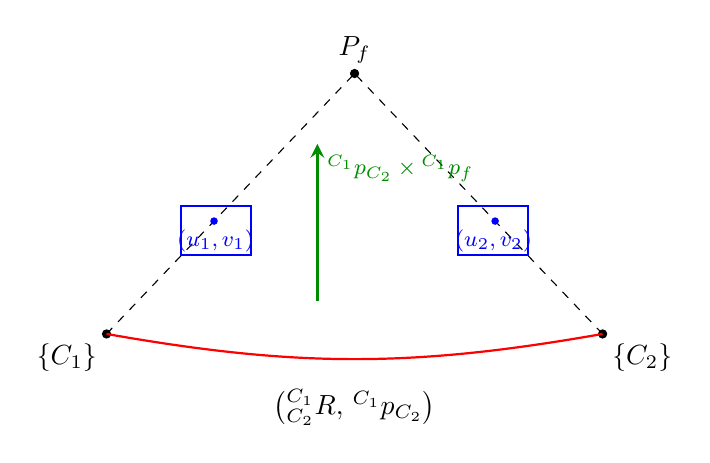
\begin{tikzpicture}[>=stealth,scale=1.05]
  \fill (3.0,3.15) circle (1.6pt) node[above] {$\vect{P}_f$};
  \draw[dashed] (0,0) -- (3.0,3.15);
  \draw[dashed] (6.0,0) -- (3.0,3.15);
  % image planes with pixels
  \draw[blue,thick] (0.90,0.95) rectangle (1.75,1.55);
  \fill[blue] (1.30,1.365) circle (1.3pt);
  \node[blue] at (1.32,1.12) {\footnotesize $(u_1,v_1)$};
  \draw[blue,thick] (4.25,0.95) rectangle (5.10,1.55);
  \fill[blue] (4.70,1.365) circle (1.3pt);
  \node[blue] at (4.68,1.12) {\footnotesize $(u_2,v_2)$};
  % camera frames
  \fill (0,0) circle (1.6pt); \node[below left] at (0,0) {$\{C_1\}$};
  \fill (6,0) circle (1.6pt); \node[below right] at (6,0) {$\{C_2\}$};
  \draw[red,thick] (0,0) to[bend right=10] (6.0,0);
  % normal of the epipolar plane (the cross product)
  \draw[->,very thick,green!55!black] (2.55,0.40) -- (2.55,2.30);
  \node[green!55!black,right] at (2.55,2.00) {\footnotesize ${}^{C_1}\vect{p}_{C_2}\times{}^{C_1}\vect{p}_f$};
  \node[below] at (3.0,-0.55) {$\big({}^{C_1}_{C_2}\vect{R},\,{}^{C_1}\vect{p}_{C_2}\big)$};
\end{tikzpicture}
\caption{Epipolar geometry: ${}^{C_1}\vect{p}_f$, ${}^{C_2}\vect{p}_f$, and the baseline ${}^{C_1}\vect{p}_{C_2}$ are coplanar, giving the essential-matrix constraint ${}^{C_1}\vect{b}\trans\vect{E}\,{}^{C_2}\vect{b} = 0$.}
\label{fig:lec03-epipolar}
\end{figure}

Why is $\vect{E}$ 5-dof? Each pair $(u_1,v_1),(u_2,v_2)$ provides 1 constraint, so we need at least \textbf{5 pairs of points} to solve $\vect{E} \Rightarrow {}^{C_1}_{C_2}\vect{R}$ (3 dof) and $\overrightarrow{{}^{C_1}\vect{p}_{C_2}}$ (2 dof, direction only). When selecting pairs of points, RANSAC (random sample consensus) comes in. Finally:
\begin{align}
\text{normalized coordinates:} \;\; & {}^{C_1}\vect{b}\trans\skewsym{{}^{C_1}\vect{p}_{C_2}}\,{}^{C_1}_{C_2}\vect{R}\,{}^{C_2}\vect{b} = 0 \;\;(\text{essential matrix}), \\
\text{pixel coordinates:} \;\; & \text{fundamental matrix}.
\end{align}
This is the \emph{motion from structure} direction.

% =====================================================================
\subsection{The full intrinsic calibration model}

The calibration geometry is the same as Fig.~\ref{fig:lec03-cammodel} (repeated here as Fig.~\ref{fig:lec03-calib}). The camera model is a composition of four functions.

\begin{figure}[H]
\centering
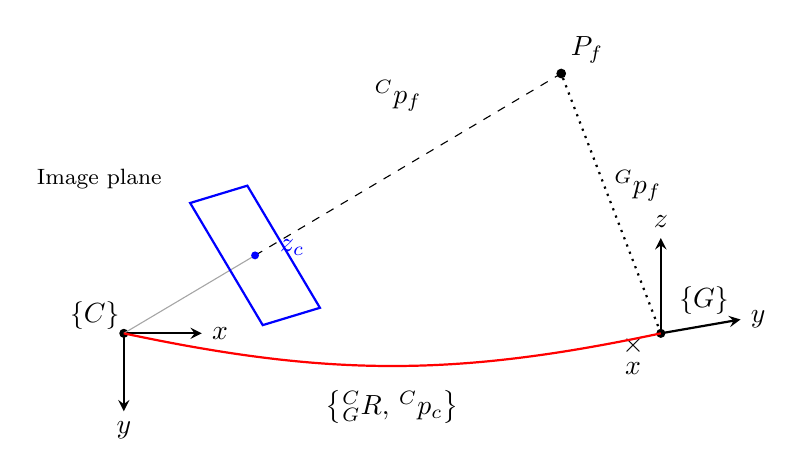
\begin{tikzpicture}[>=stealth,scale=1.1]
  \camprojscene
  \node[below] at (3.10,-0.55) {$\big\{{}^{C}_{G}\vect{R},\,{}^{C}\vect{p}_c\big\}$};
\end{tikzpicture}
\caption{The intrinsic calibration sits inside the same projection geometry: the 3D feature is transformed into $\{C\}$, projected, distorted, and mapped to pixels.}
\label{fig:lec03-calib}
\end{figure}

\paragraph{Projection and transform.}
\begin{align}
\vect{z}_n = \begin{bmatrix} c_x/c_z \\ c_y/c_z \end{bmatrix} \triangleq \vect{h}_p({}^{C}\vect{p}_f), &\qquad
{}^{C}\vect{p}_f = {}^{C}_{G}\vect{R}\trans({}^{G}\vect{p}_f - {}^{G}\vect{p}_c) \triangleq \vect{h}_t({}^{C}_{G}\vect{R},{}^{G}\vect{p}_c,{}^{G}\vect{p}_f), \\
\vect{z}_n &= \vect{h}_p\big(\vect{h}_t({}^{C}_{G}\vect{R},{}^{G}\vect{p}_c,{}^{G}\vect{p}_f)\big) + \vect{n}.
\end{align}
\paragraph{Distortion.} Radial-tangential (for example); fisheye uses the equidistant model. With $r^{2} = u_n^{2} + v_n^{2}$ and distortion parameters $\vect{x}_d = [k_1,k_2,p_1,p_2]\trans$,
\begin{align}
\begin{bmatrix} u_d \\ v_d \end{bmatrix}
= \begin{bmatrix} u_n \\ v_n \end{bmatrix}\big(1 + k_1 r^{2} + k_2 r^{4}\big)
+ \begin{bmatrix} 2 p_1 u_n v_n + p_2\,(r^{2} + 2 u_n^{2}) \\ p_1\,(r^{2} + 2 v_n^{2}) + 2 p_2 u_n v_n \end{bmatrix}, \qquad
\vect{z}_d = \begin{bmatrix} u_d \\ v_d \end{bmatrix} = \vect{h}_d(\vect{z}_n).
\end{align}
\paragraph{Intrinsics / homography.} With $\vect{x}_{in} = [f_u,f_v,c_u,c_v]$,
\begin{align}
\begin{bmatrix} u \\ v \\ 1 \end{bmatrix}
= \underbrace{\begin{bmatrix} f_u & 0 & c_u \\ 0 & f_v & c_v \\ 0 & 0 & 1 \end{bmatrix}}_{\vect{K}}\begin{bmatrix} u_d \\ v_d \\ 1 \end{bmatrix}, \qquad
\vect{z} = \begin{bmatrix} u \\ v \end{bmatrix} = \begin{bmatrix} f_u & 0 \\ 0 & f_v \end{bmatrix}\begin{bmatrix} u_d \\ v_d \end{bmatrix} + \begin{bmatrix} c_u \\ c_v \end{bmatrix} \triangleq \vect{h}_k(\vect{z}_d,\vect{x}_{in}).
\end{align}
\paragraph{Full composition.}
\begin{align}
\vect{z}_c = \vect{h}_c(\vect{x}) + \vect{n}_c
&= \vect{h}_k(\vect{z}_d,\vect{x}_{in}) + \vect{n}_c \\
&= \vect{h}_k\big(\vect{h}_d(\vect{z}_n,\vect{x}_d),\vect{x}_{in}\big) + \vect{n}_c \\
&= \vect{h}_k\big(\vect{h}_d(\vect{h}_p({}^{C}\vect{p}_f),\vect{x}_d),\vect{x}_{in}\big) + \vect{n}_c \\
&= \vect{h}_k\Big(\vect{h}_d\big(\vect{h}_p(\vect{h}_t({}^{C}_{G}\vect{R},{}^{G}\vect{p}_c,{}^{G}\vect{p}_f)),\vect{x}_d\big),\vect{x}_{in}\Big) + \vect{n}_c,
\end{align}
where $\vect{h}_k(\cdot)$ is the camera-intrinsics homography, $\vect{h}_d(\cdot)$ the distortion function, $\vect{h}_p(\cdot)$ the projection function, $\vect{h}_t(\cdot)$ the transform function, $\vect{x}_d$ the distortion parameters, and $\vect{x}_{in}=\{f_u,f_v,c_u,c_v\}$ the intrinsics. The Jacobians for calibration follow by the chain rule.

% =====================================================================
\subsection{The extrinsic (camera--IMU) calibration}

The camera and IMU sensor frames are rigidly connected (Fig.~\ref{fig:lec03-extrinsic}).

\begin{figure}[H]
\centering
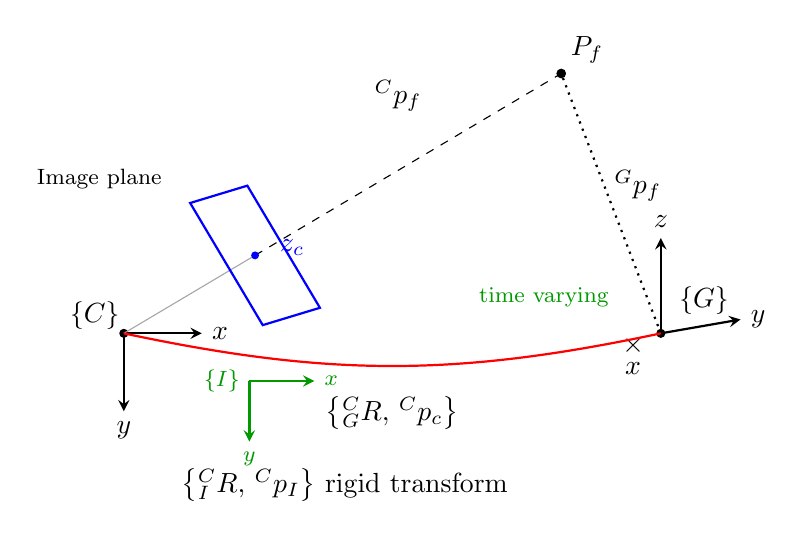
\begin{tikzpicture}[>=stealth,scale=1.1]
  \camprojscene
  % IMU frame {I}, rigidly attached near {C} (offset clearly below the camera axes)
  \draw[->,thick,green!60!black] (1.45,-0.55) -- (2.20,-0.55) node[right] {\footnotesize $x$};
  \draw[->,thick,green!60!black] (1.45,-0.55) -- (1.45,-1.25) node[below] {\footnotesize $y$};
  \node[green!60!black,left] at (1.45,-0.55) {\footnotesize $\{I\}$};
  \node[green!60!black] at (4.85,0.42) {\footnotesize time varying};
  \node[below] at (3.10,-0.62) {$\big\{{}^{C}_{G}\vect{R},\,{}^{C}\vect{p}_c\big\}$};
  \node[below] at (2.55,-1.45) {$\big\{{}^{C}_{I}\vect{R},\,{}^{C}\vect{p}_I\big\}$ rigid transform};
\end{tikzpicture}
\caption{Extrinsic calibration: the IMU frame $\{I\}$ is rigidly fixed to the camera $\{C\}$ via $\{{}^{C}_{I}\vect{R},{}^{C}\vect{p}_I\}$, while the camera-to-global transform is time varying.}
\label{fig:lec03-extrinsic}
\end{figure}

\begin{align}
\begin{bmatrix} {}^{C}\vect{p}_f \\ 1 \end{bmatrix}
&= \underbrace{\begin{bmatrix} {}^{C}_{I}\vect{R} & {}^{C}\vect{p}_I \\ \vect{0}_{1\times3} & 1 \end{bmatrix}}_{{}^{C}_{I}\vect{T}}
\underbrace{\begin{bmatrix} {}^{G}_{I}\vect{R} & {}^{G}\vect{p}_I \\ \vect{0}_{1\times3} & 1 \end{bmatrix}^{-1}}_{{}^{G}_{I}\vect{T}^{-1}}
\begin{bmatrix} {}^{G}\vect{p}_f \\ 1 \end{bmatrix}, \\
{}^{C}\vect{p}_f &= {}^{C}_{I}\vect{R}\,{}^{I}\vect{p}_f + {}^{C}\vect{p}_I = {}^{C}_{I}\vect{R}\big({}^{I}_{G}\vect{R}({}^{G}\vect{p}_f - {}^{G}\vect{p}_I)\big) + {}^{C}\vect{p}_I.
\end{align}

\paragraph{Time offset.} How do we estimate the time offset between camera and IMU? With $t_I = t_c + t_d$,
\begin{align}
\begin{bmatrix} {}^{C_{t_c}}\vect{p}_f \\ 1 \end{bmatrix} &= {}^{C}_{I}\vect{T}\cdot\big({}^{G}_{I(t+t_d)}\vect{T}\big)^{-1}\begin{bmatrix} {}^{G}\vect{p}_f \\ 1 \end{bmatrix}, \\
{}^{G}_{I(t+t_d)}\dot{\vect{T}} &= \begin{bmatrix} {}^{G}_{I}\vect{R} & {}^{G}\vect{p}_I \\ \vect{0}_{1\times3} & 1 \end{bmatrix}\begin{bmatrix} \skewsym{{}^{I}\vect{\omega}} & {}^{I}\vect{v} \\ \vect{0}_{1\times3} & 0 \end{bmatrix}.
\end{align}
which is the Jacobian for $t_d$. This is then the full calibration for the vision system.

% =====================================================================
\subsection{Point / line / plane representation}

\subsubsection{Point representation}
In $\Reals^{3}$ (closest point),
\begin{align}
\vect{P}_f = \begin{bmatrix} x \\ y \\ z \end{bmatrix} = z\begin{bmatrix} x/z \\ y/z \\ 1 \end{bmatrix} = z\begin{bmatrix} u_n \\ v_n \\ 1 \end{bmatrix}.
\end{align}
\paragraph{Inverse depth.} Store the inverse of the depth, $\lambda \triangleq 1/z$:
\begin{align}
\vect{x}_f = \begin{bmatrix} x \\ y \\ 1/z \end{bmatrix} = \begin{bmatrix} x \\ y \\ \lambda \end{bmatrix}.
\end{align}
\emph{What is the motivation to use inverse depth?} Transform the feature into a second view and divide by $z$:
\begin{align}
{}^{C_2}\vect{p}_f &= {}^{C_2}_{C_1}\vect{R}\big({}^{C_1}\vect{p}_f - {}^{C_1}\vect{p}_{C_2}\big)
= {}^{C_2}_{C_1}\vect{R}\Big(\begin{bmatrix} x \\ y \\ z \end{bmatrix} - {}^{C_1}\vect{p}_{C_2}\Big)
= {}^{C_2}_{C_1}\vect{R}\Big(z\begin{bmatrix} x/z \\ y/z \\ 1 \end{bmatrix} - {}^{C_1}\vect{p}_{C_2}\Big), \\
\frac{{}^{C_2}\vect{p}_f}{z} &= {}^{C_2}_{C_1}\vect{R}\Big(\begin{bmatrix} x/z \\ y/z \\ 1 \end{bmatrix} - \frac{1}{z}{}^{C_1}\vect{p}_{C_2}\Big)
\;\Rightarrow\;
\begin{bmatrix} {}^{C_2}x/z \\ {}^{C_2}y/z \\ {}^{C_2}z/z \end{bmatrix} = {}^{C_2}_{C_1}\vect{R}\Big(\begin{bmatrix} x\lambda \\ y\lambda \\ 1 \end{bmatrix} - \lambda\,{}^{C_1}\vect{p}_{C_2}\Big).
\end{align}
If $z\to\infty$, the feature is far away, $z\approx{}^{C_2}z \gg {}^{C_2}x,{}^{C_2}y$, then the left side tends to the bearing measurement in $\{C_2\}$:
\begin{align}
\begin{bmatrix} {}^{C_2}x/z \\ {}^{C_2}y/z \\ {}^{C_2}z/z \end{bmatrix} \approx \underbrace{\begin{bmatrix} u_{n_2} \\ v_{n_2} \\ 1 \end{bmatrix}}_{\text{measurements in } C_2} \propto {}^{C_2}_{C_1}\vect{R}\Big(\begin{bmatrix} x\lambda \\ y\lambda \\ 1 \end{bmatrix} - \lambda\,{}^{C_1}\vect{p}_{C_2}\Big).
\end{align}
The Jacobian with respect to the inverse-depth state $\tilde{\vect{x}} = [\tilde x,\tilde y,\tilde\lambda]$ is
\begin{align}
\frac{\partial[u_{n_2};v_{n_2}]}{\partial\tilde{\vect{x}}}
= \begin{bmatrix} 1 & 0 & 0 \\ 0 & 1 & 0 \end{bmatrix}\begin{bmatrix} \vect{H}_\theta & \vect{H}_p & \vect{H}_{p_f} \end{bmatrix},
\end{align}
with the three blocks
\begin{align}
\vect{H}_\theta &= \skewsym{{}^{C_2}_{C_1}\vect{R}\big([x\lambda;\,y\lambda;\,1] - \lambda\,{}^{C_1}\vect{p}_{C_2}\big)}, \qquad
\vect{H}_p = \underbrace{-\lambda\,{}^{C_2}_{C_1}\vect{R}}_{\lambda\to0}, \\
\vect{H}_{p_f} &= {}^{C_2}_{C_1}\vect{R}\big[\,\underbrace{\lambda\vect{e}_1}_{0} \;\; \underbrace{\lambda\vect{e}_2}_{0} \;\; [x;\,y;\,0]-{}^{C_1}\vect{p}_{C_2}\,\big].
\end{align}
If the feature is far away, then the rotation is improved, but the Jacobian for translation will not be improved (the $-\lambda\,{}^{C_2}_{C_1}\vect{R}$ and $\lambda\vect{e}_1,\lambda\vect{e}_2$ columns vanish as $\lambda\to0$).

\subsubsection{Plane representation}
A plane is parameterized by its normal direction and distance to the origin (Fig.~\ref{fig:lec03-plane}):
\begin{align}
\vect{\pi} = \begin{bmatrix} \vect{n}_\pi \\ d_\pi \end{bmatrix}_{4\times1}, \qquad
\vect{n}_\pi : \text{normal direction}, \quad d_\pi : \text{distance to origin}.
\end{align}
A plane is 3-dof but $\vect{\pi}$ has 4 parameters. The \emph{closest-point representation} packs both into one vector,
\begin{align}
\vect{P}_\pi = d_\pi\,\vect{n}_\pi = \begin{bmatrix} x \\ y \\ z \end{bmatrix},
\end{align}
the closest point from the plane to the origin.

\begin{figure}[H]
\centering
\begin{subfigure}[b]{0.46\textwidth}
\centering
\begin{tikzpicture}[>=stealth,scale=1.0]
  \draw[->] (0,0) -- (3.2,0) node[right] {$x$};
  \draw[->] (0,0) -- (0,3.1) node[above] {$y$};
  \fill (0,0) circle (1.2pt);
  % plane (a line in 2D)
  \draw[thick] (1.0,2.4) -- (3.0,1.0);
  % P_pi = foot of the perpendicular from the origin; d_pi and n_pi are collinear (both normal to the plane)
  \coordinate (P) at (1.456,2.081);
  \draw[dashed] (0,0) -- (P);
  \node[below right] at (0.60,0.92) {$d_\pi$};
  \fill (P) circle (1.2pt); \node[above right] at (P) {$\vect{P}_\pi$};
  \draw[->,thick] (P) -- ($(P)+(0.544,0.778)$) node[above] {$\vect{n}_\pi$};
  % right-angle mark: d_pi is perpendicular to the plane
  \draw ($(P)+(-0.103,-0.147)$) -- ($(P)+(0.044,-0.250)$) -- ($(P)+(0.147,-0.103)$);
\end{tikzpicture}
\caption{plane: $\vect{n}_\pi$, $d_\pi$, foot $\vect{P}_\pi$}
\label{fig:lec03-plane}
\end{subfigure}
\hfill
\begin{subfigure}[b]{0.50\textwidth}
\centering
\begin{tikzpicture}[>=stealth,scale=0.95]
  % plane (a line); outward normal points up-right at 45 deg
  \coordinate (Pa) at (5.2,1.5);
  \coordinate (Pb) at (2.8,3.9);
  \draw[thick] (Pa) -- (Pb);
  % a marked point on the plane carrying the normal
  \coordinate (Pn) at (3.0,3.75);
  \fill (Pn) circle (1.2pt); \node[left] at (Pn) {$\vect{P}_\pi$};
  \draw[->,thick] (Pn) -- ($(Pn)+(0.6,0.6)$) node[above right] {$\vect{n}$};
  % camera frame {C} (small triad)
  \coordinate (C) at (0.8,1.0);
  \fill (C) circle (1.2pt);
  \draw[->] (C) -- ($(C)+(0.55,0.22)$); \draw[->] (C) -- ($(C)+(-0.15,0.5)$);
  \node[below] at (C) {$\{C\}$};
  % IMU frame {I} (green triad, rigidly attached)
  \coordinate (I) at (2.1,0.65);
  \fill[green!55!black] (I) circle (1.2pt);
  \draw[->,green!55!black] (I) -- ($(I)+(0.55,0.22)$); \draw[->,green!55!black] (I) -- ($(I)+(-0.15,0.5)$);
  \node[green!55!black,below] at (I) {$\{I\}$};
  % perpendicular distances to the plane (parallel, along the normal, distinct feet)
  \coordinate (Fc) at (3.249,3.449);
  \coordinate (Fi) at (4.049,2.649);
  \draw[dashed] (C) -- (Fc); \node[above left] at (1.95,2.35) {${}^{C}d_\pi$};
  \draw[dotted,thick] (I) -- (Fi); \node[below right] at (3.35,1.80) {${}^{I}d_\pi$};
  % right-angle marks at the feet
  \draw ($(Fc)+(-0.113,-0.113)$) -- ($(Fc)+(-0.226,0)$) -- ($(Fc)+(-0.113,0.113)$);
  \draw ($(Fi)+(-0.113,-0.113)$) -- ($(Fi)+(-0.226,0)$) -- ($(Fi)+(-0.113,0.113)$);
\end{tikzpicture}
\caption{transfer the plane $\{C\}\to\{I\}$}
\label{fig:lec03-planetransfer}
\end{subfigure}
\caption{Plane representation (a) and its transfer between the camera and IMU frames (b).}
\end{figure}

\paragraph{Transfer $\{C\}\to\{I\}$.} For ${}^{C}\vect{p}_\pi \leftrightarrow {}^{I}\vect{p}_\pi$ (Fig.~\ref{fig:lec03-planetransfer}),
\begin{align}
\begin{cases}
{}^{I}\vect{n}_\pi = {}^{I}_{C}\vect{R}\,{}^{C}\vect{n}_\pi & \Rightarrow \text{normal direction} \\[2pt]
{}^{I}d_\pi = {}^{C}d_\pi - {}^{C}\vect{n}_\pi\trans\cdot{}^{C}\vect{p}_I & \Rightarrow \text{origin to plane}
\end{cases}
\end{align}
Hence, using ${}^{I}d_\pi = {}^{C}d_\pi - {}^{C}\vect{p}_I\trans\,{}^{C}\vect{n}_\pi$ and ${}^{C}\vect{p}_I = -{}^{C}_{I}\vect{R}\,{}^{I}\vect{p}_C$ (so $-{}^{C}\vect{p}_I\trans = {}^{I}\vect{p}_C\trans\,{}^{I}_{C}\vect{R}$),
\begin{align}
\begin{bmatrix} {}^{I}\vect{n}_\pi \\ {}^{I}d_\pi \end{bmatrix} = \begin{bmatrix} {}^{I}_{C}\vect{R} & \vect{0}_{3\times1} \\ -{}^{C}\vect{p}_I\trans & 1 \end{bmatrix}\begin{bmatrix} {}^{C}\vect{n}_\pi \\ {}^{C}d_\pi \end{bmatrix}
= \begin{bmatrix} {}^{I}_{C}\vect{R} & \vect{0}_{3\times1} \\ {}^{I}\vect{p}_C\trans\,{}^{I}_{C}\vect{R} & 1 \end{bmatrix}\begin{bmatrix} {}^{C}\vect{n}_\pi \\ {}^{C}d_\pi \end{bmatrix}.
\end{align}
The transformation chain is therefore
\begin{align}
{}^{G}\vect{p}_\pi \to ({}^{C}\vect{n}_\pi,{}^{C}d_\pi) \to ({}^{I}_{C}\vect{R},{}^{I}\vect{p}_C) \to ({}^{I}\vect{n}_\pi,{}^{I}d_\pi) \to {}^{I}\vect{p}_\pi.
\end{align}

\subsubsection{Line representation}
How do we represent a 3D line (Fig.~\ref{fig:lec03-line3d})? For a line $L$: $\vect{v}_e$ is the 3D direction, $d_L$ is the distance from the origin to the line, and $\vect{n}_e$ is the normal direction of the plane (through the line and the origin).

\begin{figure}[H]
\centering
\begin{tikzpicture}[>=stealth,scale=1.2]
  % 3D axes
  \draw[->] (0,0) -- (0,2.7) node[above] {$z$};
  \draw[->] (0,0) -- (2.8,0.2) node[right] {$y$};
  \draw[->] (0,0) -- (-1.3,-0.95) node[below left] {$x$};
  \fill (0,0) circle (1.2pt);
  % plane through the line and the origin (faint triangle)
  \coordinate (A) at (0.40,1.95);
  \coordinate (B) at (2.45,1.60);
  \draw[gray!45] (0,0) -- (A) -- (B) -- cycle;
  % the line L (red)
  \draw[red,very thick] (A) -- (B);
  \node[above left,black] at (0.62,1.92) {$L$};
  % anchor M = closest point of the line to the origin (foot of d_L)
  \coordinate (M) at (1.22,1.81);
  % orthonormal frame {n_e, v_e, <n_e>x v_e} at M
  \draw[->,thick,blue] (M) -- ($(M)+(1.00,-0.17)$) node[right] {$\vect{v}_e$};            % along the line
  \draw[->,thick,blue] (M) -- ($(M)+(0.30,0.98)$) node[above] {$\vect{n}_e$};               % plane normal
  \draw[->,thick,blue] (M) -- ($(M)+(-0.80,-0.42)$) node[below left] {\footnotesize $\skewsym{\vect{n}_e}\vect{v}_e$};
  % perpendicular distance d_L from origin to the line
  \draw[dashed] (0,0) -- (M); \node[right] at (0.50,0.78) {$d_L$};
\end{tikzpicture}
\caption{3D line $L$: direction $\vect{v}_e$, plane normal $\vect{n}_e$, third axis $\skewsym{\vect{n}_e}\vect{v}_e$, and perpendicular distance $d_L$ from the origin.}
\label{fig:lec03-line3d}
\end{figure}

We can represent a line with $\{\vect{n}_e,\vect{v}_e,d_L\}$, where
\begin{align}
\vect{R}_L = \begin{bmatrix} \vect{n}_e & \vect{v}_e & \skewsym{\vect{n}_e}\vect{v}_e \end{bmatrix} \;\text{(a rotation matrix)}, \qquad d_L \;\text{(a distance scalar)}.
\end{align}
So $L : \{\vect{R}_L,d_L\} : \{\bar{\vect{q}}_L,d_L\}$, packed as the 4D vector $\vect{P}_L = \bar{\vect{q}}_L\cdot d_L$, with the error states in Euclidean space. Then
\begin{align}
\vect{P}_L = \hat{\vect{P}}_L + \tilde{\vect{P}}_L
&= \bar{\vect{q}}_L\cdot d_L = \hat{\bar{\vect{q}}}_L \otimes \delta\vect{q}_L\cdot(\hat d_L + \tilde d_L) \\
\Leftrightarrow\; \hat{\vect{P}}_L + \tilde{\vect{P}}_L &= \hat{\bar{\vect{q}}}_L \otimes \begin{bmatrix} 1 \\ \tfrac12\delta\vect{\theta}_L \end{bmatrix}(\hat d_L + \tilde d_L) \\
&= \hat{\bar{\vect{q}}}_L \otimes \begin{bmatrix} \hat d_L + \tilde d_L \\ \tfrac12\hat d_L\,\delta\vect{\theta}_L \end{bmatrix} \\
&= \hat{\bar{\vect{q}}}_L \otimes \Big(\begin{bmatrix} \hat d_L \\ \vect{0}_{3\times1} \end{bmatrix} + \begin{bmatrix} 1 & \vect{0} \\ \vect{0} & \tfrac12\hat d_L\vect{I}_3 \end{bmatrix}\begin{bmatrix} \tilde d_L \\ \delta\vect{\theta}_L \end{bmatrix}\Big),
\end{align}
so that, with $\lfloor\hat{\bar{\vect{q}}}_L\rfloor_L$ the left quaternion-product matrix,
\begin{empheq}[box=\fbox]{align}
\tilde{\vect{P}}_L = \big\lfloor\hat{\bar{\vect{q}}}_L\big\rfloor_L\begin{bmatrix} 1 & \vect{0} \\ \vect{0} & \tfrac12\hat d_L\vect{I}_3 \end{bmatrix}\begin{bmatrix} \tilde d_L \\ \delta\vect{\theta}_L \end{bmatrix}.
\end{empheq}

\paragraph{A few discussions on lines with cameras.}

\textbf{(1) How to project a 3D line to a 2D line in the image?} Given a line $\{\vect{n}_e,\vect{v}_e,d_L\}$ and camera parameters $f_u,f_v,c_u,c_v$ (Fig.~\ref{fig:lec03-lineproj}):
\begin{align}
\begin{bmatrix} u_n \\ v_n \\ 1 \end{bmatrix} \sim \underbrace{\begin{bmatrix} f_u & 0 & c_u \\ 0 & f_v & c_v \\ 0 & 0 & 1 \end{bmatrix}}_{\vect{K}}\underbrace{\begin{bmatrix} x \\ y \\ z \end{bmatrix}}_{\vect{p}_f}, \qquad
\underbrace{\vect{p}}_{\text{pixel on image}} \sim \vect{K}\,\vect{p}_f.
\end{align}
Every $\vect{p}_f$ on the line lies in the plane through the line and the origin, so $\vect{p}_f\trans\vect{n}_e = 0$. With $\vect{p}_f \sim \vect{K}^{-1}\vect{p}$,
\begin{align}
(\vect{K}^{-1}\vect{p})\trans\vect{n}_e = 0 \;\Rightarrow\; \vect{p}\trans\vect{K}^{-\top}\vect{n}_e = 0 \;\Rightarrow\; \vect{n}_e\trans\vect{K}^{-1}\vect{p} = 0 \;\Rightarrow\; (\vect{K}^{-\top}\vect{n}_e)\trans\vect{p} = 0,
\end{align}
so the 2D image line is
\begin{align}
\vect{l} = \vect{K}^{-\top}\vect{n}_e, \qquad \vect{p} \text{ is every pixel on the line}.
\end{align}

\begin{figure}[H]
\centering
\begin{subfigure}[b]{0.46\textwidth}
\centering
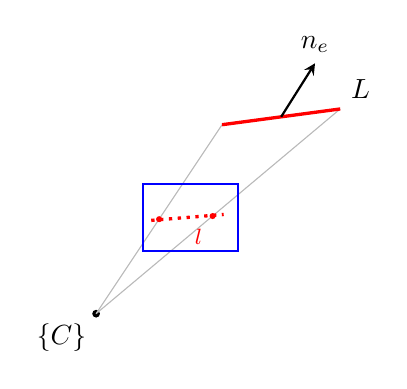
\begin{tikzpicture}[>=stealth,scale=1.0]
  \fill (0,0) circle (1.4pt); \node[below left] at (0,0) {$\{C\}$};
  % the 3D line L and the two sight rays from {C} to its endpoints
  \coordinate (A) at (1.6,2.4);
  \coordinate (B) at (3.1,2.6);
  \draw[gray!55] (0,0) -- (A); \draw[gray!55] (0,0) -- (B);
  \draw[red,very thick] (A) -- (B) node[above right,black] {$L$};
  % normal of the plane through {C} and L
  \draw[->,thick] (2.35,2.5) -- (2.78,3.18) node[above] {$\vect{n}_e$};
  % image plane
  \draw[blue,thick] (0.6,0.8) rectangle (1.8,1.65);
  % projected image line l = where the (C,L) plane meets the image plane
  \fill[red] (0.80,1.20) circle (1.1pt); \fill[red] (1.48,1.24) circle (1.1pt);
  \draw[red,dotted,very thick] (0.70,1.185) -- (1.62,1.26);
  \node[red] at (1.30,0.98) {\footnotesize $\vect{l}$};
\end{tikzpicture}
\caption{project 3D line $\to$ image line $\vect{l}=\vect{K}^{-\top}\vect{n}_e$}
\label{fig:lec03-lineproj}
\end{subfigure}
\hfill
\begin{subfigure}[b]{0.50\textwidth}
\centering
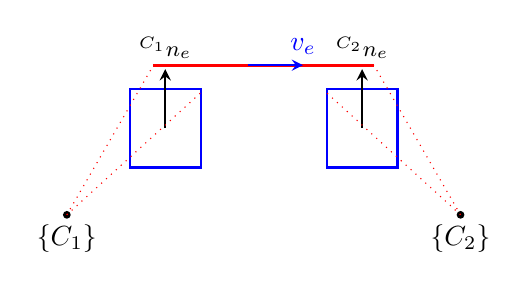
\begin{tikzpicture}[>=stealth,scale=1.0]
  \fill (0,0) circle (1.4pt); \node[below] at (0,0) {$\{C_1\}$};
  \fill (5.0,0) circle (1.4pt); \node[below] at (5.0,0) {$\{C_2\}$};
  % image planes
  \draw[blue,thick] (0.8,0.6) rectangle (1.7,1.6);
  \draw[blue,thick] (3.3,0.6) rectangle (4.2,1.6);
  % 3D line viewed from both (red), shared direction v_e
  \draw[red,very thick] (1.1,1.9) -- (3.9,1.9);
  \draw[->,thick,blue] (2.3,1.9) -- (3.0,1.9) node[above] {$\vect{v}_e$};
  % per-image normals
  \draw[->,thick] (1.25,1.1) -- (1.25,1.85) node[above] {\footnotesize ${}^{C_1}\vect{n}_e$};
  \draw[->,thick] (3.75,1.1) -- (3.75,1.85) node[above] {\footnotesize ${}^{C_2}\vect{n}_e$};
  % rays from the camera centres
  \draw[red,dotted] (0,0) -- (1.1,1.9); \draw[red,dotted] (0,0) -- (1.7,1.55);
  \draw[red,dotted] (5.0,0) -- (3.9,1.9); \draw[red,dotted] (5.0,0) -- (3.3,1.55);
\end{tikzpicture}
\caption{transfer a line $\{C_1\}\to\{C_2\}$}
\label{fig:lec03-linetransfer}
\end{subfigure}
\caption{Lines with cameras: projecting a 3D line to a 2D image line (a) and transferring a line between two camera frames (b).}
\end{figure}

\textbf{(2) How to transfer a line from frame $\{C_1\}$ to $\{C_2\}$?} (Fig.~\ref{fig:lec03-linetransfer}) The line $L$ is given by ${}^{C_1}\vect{n}_e$, ${}^{C_1}\vect{v}_e$, ${}^{C_1}d_L$ in $\{C_1\}$ and by ${}^{C_2}\vect{n}_e$, ${}^{C_2}\vect{v}_e$, ${}^{C_2}d_L$ in $\{C_2\}$. Assume ${}^{C_1}\vect{p}_f$ is a point on $L$; then its moment about the origin is
\begin{align}
\skewsym{{}^{C_1}\vect{p}_f}\,{}^{C_1}\vect{v}_e = {}^{C_1}\vect{n}_e\,{}^{C_1}d_L.
\end{align}
The direction transforms by rotation only, and the point by the full rigid transform:
\begin{align}
{}^{C_2}\vect{v}_e = {}^{C_2}_{C_1}\vect{R}\,{}^{C_1}\vect{v}_e, \qquad
{}^{C_2}\vect{p}_f = {}^{C_2}_{C_1}\vect{R}\,{}^{C_1}\vect{p}_f + {}^{C_2}\vect{p}_{C_1}.
\end{align}
Hence the moment in $\{C_2\}$ is
\begin{align}
\skewsym{{}^{C_2}\vect{p}_f}\,{}^{C_2}\vect{v}_e
= \skewsym{{}^{C_2}_{C_1}\vect{R}\,{}^{C_1}\vect{p}_f + {}^{C_2}\vect{p}_{C_1}}\,{}^{C_2}_{C_1}\vect{R}\,{}^{C_1}\vect{v}_e
= {}^{C_2}\vect{n}_e\,{}^{C_2}d_L.
\end{align}
Using $\skewsym{\vect{R}\vect{a}}\vect{R} = \vect{R}\skewsym{\vect{a}}$ on the first term,
\begin{align}
{}^{C_2}_{C_1}\vect{R}\,\skewsym{{}^{C_1}\vect{p}_f}\,{}^{C_1}\vect{v}_e + \skewsym{{}^{C_2}\vect{p}_{C_1}}\,{}^{C_2}_{C_1}\vect{R}\,{}^{C_1}\vect{v}_e = {}^{C_2}\vect{n}_e\,{}^{C_2}d_L,
\end{align}
and substituting the moment identity ${}^{C_1}\vect{n}_e\,{}^{C_1}d_L = \skewsym{{}^{C_1}\vect{p}_f}\,{}^{C_1}\vect{v}_e$,
\begin{align}
\begin{bmatrix} {}^{C_2}_{C_1}\vect{R} & \skewsym{{}^{C_2}\vect{p}_{C_1}}\,{}^{C_2}_{C_1}\vect{R} \end{bmatrix}\begin{bmatrix} {}^{C_1}\vect{n}_e\,{}^{C_1}d_L \\ {}^{C_1}\vect{v}_e \end{bmatrix} = {}^{C_2}\vect{n}_e\,{}^{C_2}d_L.
\end{align}
Stacking the moment and the direction (${}^{C_2}\vect{v}_e = {}^{C_2}_{C_1}\vect{R}\,{}^{C_1}\vect{v}_e$) gives the full line transfer:
\begin{empheq}[box=\fbox]{align}
\begin{bmatrix} {}^{C_2}\vect{n}_e\,{}^{C_2}d_L \\ {}^{C_2}\vect{v}_e \end{bmatrix}
= \begin{bmatrix} {}^{C_2}_{C_1}\vect{R} & \skewsym{{}^{C_2}\vect{p}_{C_1}}\,{}^{C_2}_{C_1}\vect{R} \\ \vect{0}_{3} & {}^{C_2}_{C_1}\vect{R} \end{bmatrix}\begin{bmatrix} {}^{C_1}\vect{n}_e\,{}^{C_1}d_L \\ {}^{C_1}\vect{v}_e \end{bmatrix}.
\end{empheq}
